\begin{name}
	{\tenchude}
	{\tendethi}
	{\tentruong}
	{\thoigian}
\end{name}
\Opensolutionfile{ansbook}[ans/ansbookDe4]
\TN
\Opensolutionfile{ans}[ans/ansDe4-TN1]
\begin{ex}%[1D6N3-2]
	Tập xác định của hàm số $y = (x-1)^{\tfrac{1}{3}}$ là
	\choice
	{$ [1; +\infty)$}
	{\True$ (1; +\infty)$}
	{ $\mathbb{R}$}
	{ Một đáp án khác}
	\loigiai{Điều kiện xác  định $x-1 > 0 \Leftrightarrow x > 1$.\\
	Vậy tập xác định $\mathscr{D}= (1; +\infty)$.}
	\end{ex}

	\begin{ex}%[1D6N2-2]
		Cho $a>0$, $a\neq1$. Chọn khẳng định đúng trong các khẳng định sau
		\choice
		{$\log_a a^3=a^3$}
		{$\log_a a^3=3+a$}
		{\True $\log_a a^3=3$}
		{$\log_a a^3=3a$}
		\loigiai{
		Do $\log_a a^3=3\log_a a=3$.
		}
		\end{ex}

		\begin{ex}%[10-11EX-GK2-2425]%[Trần Hưng]%[1D6N3-3]
			\immini{
			Hàm số nào dưới đây có đồ thị như hình vẽ?
			\choice
			{\True $y=\log _{3}x$}
			{$y=3^{x-3}$}
			{$y=\log _{\tfrac{1}{3}}x$}
			{$y=\left(\frac{1}{3}\right)^{x}$}
			}{
			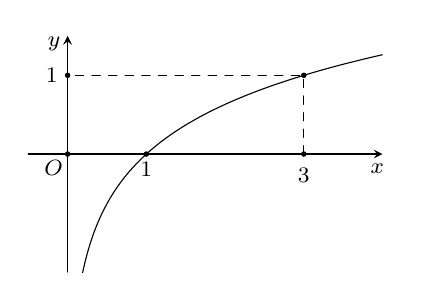
\begin{tikzpicture}[scale=1, font=\footnotesize, line join=round, line cap=round, >=stealth]
			\def \xmin{-.5}
			\def \xmax{4}
			\def \ymin{-1.5}
			\def \ymax{1.5}
			\draw[->] (\xmin,0)--(\xmax,0) node[shift=(-110:0.2)] {$x$};
			\draw[->] (0,\ymin)--(0,\ymax) node[shift=(-150:0.2)] {$y$};
			\fill (0,0) circle(1pt) node[shift=(-135:0.25)]{$O$}
			(1,0) circle(1pt) node[shift=(-90:0.2)]{$1$}
			(3,0) circle(1pt) node[shift=(-90:0.27)]{$3$}
			(0,1) circle(1pt) node[shift=(180:0.2)]{$1$}
			(3,1) circle(1pt)
			;
			\draw[dashed] (3,0)|-(0,1);
			\clip (\xmin,\ymin) rectangle (\xmax,\ymax);
			\draw[smooth,samples=100,domain=.1:\xmax] plot(\x,{ln(\x)/ln(3)});
			\end{tikzpicture}
			}
			\loigiai{
			Dựa vào đồ thị hàm số, suy ra $y=\log _{3}x$.
			}
			\end{ex}

\begin{ex}%[10-11-EX-GK2-2425]%[Trần Tony]%[1H8N1-1]
Trong các mệnh đề sau, mệnh đề nào đúng?
\choice
{Một đường thẳng vuông góc với một trong hai đường thẳng vuông góc với nhau thì song song với đường thẳng còn lại}
{Hai đường thẳng cùng vuông góc với một đường thẳng thì song song với nhau}
{Hai đường thẳng cùng vuông góc với một đường thẳng thì vuông góc với nhau}
{\True Một đường thẳng vuông góc với một trong hai đường thẳng song song thì vuông góc với đường thẳng còn lại}
\loigiai{
Nếu $a\parallel b$ thì $(a,c)=(b,c)$.\\
Do đó, mệnh đề đúng là \lq\lq Một đường thẳng vuông góc với một trong hai đường thẳng song song thì vuông góc với đường thẳng còn lại\rq\rq.
}
\end{ex}

\begin{ex}%[1H8N3-1]%[Dự án đề kiểm tra Toán 11 CHKII NH23-24- Ngô Tất Thành]%[THPT Phạm Văn Sáng - Tp HCM]
	Cho hình chóp $S.ABCD$ có $SD \perp (ABCD)$. Hình chiếu vuông góc của $S$ lên $(ABCD)$ là điểm
	\choice
	{$A$}
	{$C$}
	{$B$}
	{\True $D$}
	\loigiai{
	Hình chiếu vuông góc của $S$ lên $(ABCD)$ là điểm D vì $SD \perp (ABCD)$.
	}
	\end{ex}

\begin{ex}%[1H8N4-1]
Hãy chọn khẳng định đúng.
\choice
{Nếu hai mặt phẳng vuông góc với nhau thì bất cứ đường nào nằm trong mặt phẳng này cũng vuông góc với mặt phẳng kia}
{Nếu hai mặt phẳng cùng vuông góc với mặt phẳng thứ ba thì giao tuyến của chúng vuông góc với mặt phẳng thứ ba đó}
{\True Nếu mặt phẳng này chứa một đường thẳng mà đường thẳng đó vuông góc với mặt phẳng kia thì hai mặt phẳng đó vuông góc với nhau}
{Nếu mặt phẳng này chứa một đường thẳng mà đường thẳng đó vuông góc với một đường thẳng nằm trong mặt phẳng kia thì hai mặt phẳng đó vuông góc với nhau}
\loigiai{
Nếu mặt phẳng này chứa một đường thẳng mà đường thẳng đó vuông góc với mặt phẳng kia thì hai mặt phẳng đó vuông góc với nhau.
}
\end{ex}

\begin{ex}%[1H8N6-1]
% \immini[thm]{
	Cho hình chóp $ S.ABCD $ có $ SB\perp (ABCD)$, góc giữa đường thẳng $ SD $ và mặt phẳng $(ABCD)$ là góc nào sau đây?
\choice
{\True $\widehat{SDB}$}
{$\widehat{DSB}$}
{$\widehat{SDC}$}
{$\widehat{SDA}$}
% }
% {\begin{tikzpicture}[scale=0.5, font=\footnotesize,line join=round, line cap=round,>=stealth]
% \tkzDefPoints{0/0/B,-2/-2/A,5/0/C,3/-2/D,0/5/S}
% \tkzDrawSegments(S,A S,C S,D A,D D,C)
% \tkzDrawSegments[dashed](S,B A,B B,C)
% \tkzDrawPoints[fill=black,size=3](A,B,C,D,S)
% \tkzLabelPoints[below](A,D)
% \tkzLabelPoints[above](S)
% \tkzLabelPoints[left](B)
% \tkzLabelPoints[right](C)

% \end{tikzpicture}}
\loigiai{
\immini{Vì $ SB\perp (ABCD)$ nên hình chiếu của $ SD $ lên $(ABCD)$ là $ BD $ nên góc giữa đường thẳng $ SD $ và mặt phẳng $(ABCD)$ là $\widehat{SDB}$.}
{\begin{tikzpicture}[scale=0.5, font=\footnotesize,line join=round, line cap=round,>=stealth]
\tkzDefPoints{0/0/B,-2/-2/A,5/0/C,3/-2/D,0/5/S}
\tkzDrawSegments(S,A S,C S,D A,D D,C)
\tkzDrawSegments[dashed](S,B A,B B,C B,D)
\tkzDrawPoints[fill=black,size=3](A,B,C,D,S)
\tkzLabelPoints[below](A,D)
\tkzLabelPoints[above](S)
\tkzLabelPoints[left](B)
\tkzLabelPoints[right](C)
\tkzMarkAngles[size=1cm](S,D,B)

\end{tikzpicture}}
}
\end{ex}

\begin{ex}%[1H8N7-1]
Nếu một khối lăng trụ đứng có diện tích đáy bằng $B$ và cạnh bên bằng $h$ thì có thể tích là
\choice
{$\dfrac{1}{2} B h$}
{$\dfrac{1}{3} B h$}
{$3 B h$}
{\True $Bh$}
\loigiai{
Thể tích khối lăng trụ đứng là $V=Bh$.
}
\end{ex}

\begin{ex}%[1D9N1-1]%[Dự án đề kiểm tra Toán 11 GHKI NH23-24- Tổng Nguyễn]%[THPT Phạm Phú Thứ - Đà Nẵng]
Cho $A$ và $B$ là hai biến cố độc lập. Cặp biến cố nào sau đây là độc lập?
\choice
{$A$ và $\overline{A}$}
{$B$ và $\overline{B}$}
{\True $A$ và $\overline{B}$}
{$AB$ và $\overline{A} \overline{B}$}
\loigiai{ Vì $A$ và $B$ là hai biến cố độc lập nên $A$ và $\overline{B}$ độc lập.
}
\end{ex}

\begin{ex}%[1D9N2-1]%[Dự án đề kiểm tra Toán 11 HK II NH23-24 - Nguyễn Thành Sơn]%[THPT Nguyễn Thái Bình - Tp.HCM]
Xét một phép thử có không gian mẫu là $\Omega$ và $A$ là một biến cố của phép thử đó. Phát biểu nào dưới đây là \textbf{sai}?
\choice
{$0 \leq \mathrm{P}(A) \leq 1$}
{\True $\mathrm{P}(A)=0$ khi và chi khi $A$ là biến cố chắc chắn}
{Xác suất của biến cố $A$ là số $\mathrm{P}(A)=\dfrac{n(A)}{n(\Omega)}$}
{$\mathrm{P}(A)=1-\mathrm{P}(\overline{A})$}
\loigiai{$\mathrm{P}(A)=1$ khi và chỉ khi $A$ là biến cố chắc chắn.\\ Do đó $\mathrm{P}(A)=0$ khi và chỉ khi $A$ là biến cố chắc chắn là phát biểu \textbf{sai}.
}
\end{ex}

\begin{ex}%[1D7N1-1]%[Dự án đề kiểm tra Toán 11 CKII NH23-24- Hoàng Vũ]%[THPT TRẦN ĐẠI NGHĨA - HCM]
Cho hàm số $y=f(x)$ có đạo hàm trên $\mathbb{R}$ thỏa mãn $f'(6)=2$. Giá trị biểu thức $\lim\limits_{x\rightarrow 6}\dfrac{f(x)-f(6)}{x-6}$ bằng
\choice
{$\dfrac{1}{3}$}
{\True$2$}
{$12$}
{$\dfrac{1}{2}$}
\loigiai{
Ta có $\lim\limits_{x\rightarrow 6}\dfrac{f(x)-f(6)}{x-6}=f'(6)=2$
}
\end{ex}

\begin{ex}%[1D7N2-8]
	Xét chuyển động thẳng xác định bởi phương trình $s=s(t)$ với $s=s(t)$ là một hàm số có đạo hàm; $v=v(t)$ và $a=a(t)$ lần lượt là vận tốc tức thời và gia tốc tức thời của chuyển động tại thời điểm $t$. Khi đó
	\choice
	{$a''(t)=v(t)$}
	{$v''(t)=a(t)$}
	{$a''(t)=s(t)$}
	{\True $s''(t)=a(t)$}
	\loigiai{
	Mối liên hệ giữa công thức tính quãng đường, vận tốc và gia tốc chuyển động thẳng tại thời điểm $t$ là $s'(t)=v(t)$, $s''(t)=a(t)$.
	}
	\end{ex}
\Closesolutionfile{ans}

\TNTF
\Opensolutionfile{ans}[ans/ansDe4-TN2]
\begin{ex}%[1D7H1-1]
	Dùng định nghĩa tìm đạo hàm của hàm số $y=x^2+1$ trên tập xác định. \\Khi đó các mệnh đề sau đúng hay sai?
	\choiceTF
	{$f'(x_0)=\dfrac{f(x)-f(x_0)}{x-x_0}$}
	{\True $f'(x_0)=\lim _{x \to x_0} \dfrac{f(x)-f(x_0)}{x-x_0}=2 x_0$}
	{\True $f'(2)=4$}
	{\True $f'(2)+f'(-2)=0$}
	\loigiai{
	\begin{itemchoice}
	\itemch Vì $f'(x_0)=\lim _{x \to x_0} \dfrac{f(x)-f(x_0)}{x-x_0}$.
	\itemch Ta có \begin{eqnarray*}
	f'(x_0)=\lim _{x \to x_0} \dfrac{f(x)-f(x_0)}{x-x_0}=\lim _{x \to x_0} \dfrac{x^{2}+1-(x_0^{2}+1)}{x-x_0}&=&\lim _{x \to x_0}(x+x_0)\\
	&=&2 x_0.
	\end{eqnarray*}
	\itemch Ta có $f'(x_0)=2 x_0$ nên $f'(2)=4$.
	\itemch Ta có $f'(x_0)=2 x_0$ nên $f'(2)+f'(-2)=4-4=0$.
	\end{itemchoice}
	}
	\end{ex}

\begin{ex}%[Dự Án Giảng 12 4 in 1, Lê Văn Toàn]%[1D7H2-1]
Cho hàm số $y=x^{4}-4x^{2}+3 \sqrt{x}+2-\dfrac{1}{x}$. Khi đó
\choiceTFt
{\True $y'(1)=-\dfrac{3}{2}$}
{Đồ thị của hàm số $y'$ đi qua điểm $A\left(1;\dfrac{3}{2}\right)$}
{\True $y'(4)=\dfrac{3597}{16}$}
{\True Điểm $M$ thuộc đồ thị $(C)$ của hàm số $y=x^{4}-4x^{2}+3\sqrt{x}+2-\dfrac{1}{x}$ có hoành độ $x_{0}=1$. Khi đó, tiếp tuyến của $(C)$ tại $M$ vuông góc với đường thẳng $y=\dfrac{2}{3}x$}
\loigiai{
Ta có $y'=4 \cdot x^{3}-4 \cdot 2 \cdot x+3 \cdot \dfrac{1}{2 \sqrt{x}}+0-\left(-\dfrac{1}{x^{2}}\right)=4x^{3}-8x+\dfrac{3}{2 \sqrt{x}}+\dfrac{1}{x^{2}}$.
\begin{itemchoice}
\itemch $y'(1)=-\dfrac{3}{2}$.
\itemch Đồ thị của hàm số $y'=4x^{3}-8x+\dfrac{3}{2 \sqrt{x}}+\dfrac{1}{x^{2}}$ đi qua điểm $A\left(1;-\dfrac{3}{2}\right)$.
\itemch $y'(4)=\dfrac{3597}{16}$.
\itemch Ta có $M(1;1)$ thuộc đồ thị $(C)$.\\
Tiếp tuyến tại $M$ có hệ số góc $k=-\dfrac{3}{2}$ vuông góc với đường thẳng $y=\dfrac{2}{3}x$.
\end{itemchoice}
}
\end{ex}
\Closesolutionfile{ans}

\TNSA
\Opensolutionfile{ans}[ans/ansDe4-TN3]
\begin{ex}%[1D6H4-3]%[Dự án đề kiểm tra Toán 11 HKII NH23-24 - Dot 15- Xuan Vy Pham]%[THPT Nguyễn Du - TP.HCM]
Có bao nhiêu số nguyên $x$ thỏa bất phương trình $\log_3 (x+3) \le 2$.
\shortans{$9$}
\loigiai{

Điều kiện $x+3>0 \Leftrightarrow x>-3$.

Ta có $\log_3 (x+3) \le 2 \Leftrightarrow x+3 \le 3^2 \Leftrightarrow x \le 6$.

Kết hợp với điều kiện ta được nghiệm của bất phương trình là $ -3 < x \le 6$.

Mà $x$ là số nguyên nên $x \in \left\{-2;-1;0;1;2;3;4;5;6\right\}$.

Do đó có $9$ số nguyên thỏa bất phương trình đã cho.
}
\end{ex}

\begin{ex}%[1H8H5-2]%[tex hóa ck2-form 2025-dot 2-Nguyễn Chín Em]
Cho hình chóp $ S.ABCD$ có đáy $ ABCD$ là hình chữ nhật, $ AB=a, AD=2a\sqrt 3 $. Cạnh bên $ SA$ vuông góc với đáy, biết tam giác $ SAD$ có diện tích $ S=3a^2$. Khi $ a=\sqrt{51}$ thì khoảng cách từ $ C$ đến $\left(SBD\right)$ bằng bao nhiêu?
\shortans{$6$}
\loigiai{
\immini{
Do $S_{SAD}=3a^2=\dfrac{1}{2}\cdot SA\cdot AD\Rightarrow SA=\dfrac{6a^2}{2a\sqrt 3}=a\sqrt 3 $.\\
Mặt khác ta có $\mathrm{d}\left(C,\left(SBD\right)\right)=\mathrm{d}\left(A,\left(SBD\right)\right)$.\\
Kẻ $ AH\perp BD$ tại $H$, $AK\perp SH$ tại $K$.
\begin{align*}
&\Rightarrow d\left(A,\left(SBD\right)\right)=AK\\
& BD=\sqrt{A{B^2}+A{D^2}}=a\sqrt{13}\\
&\Rightarrow AH=\dfrac{AB\cdot AD}{BD}=\dfrac{a\cdot 2a\sqrt 3}{a\sqrt{13}}=\dfrac{2a\sqrt{39}}{13}\\
&\Rightarrow AK=\dfrac{SA\cdot AH}{\sqrt{S{A^2}+A{H^2}}}=\dfrac{a\sqrt 3 \cdot \dfrac{2a\sqrt{39}}{13}}{\sqrt{\left(a\sqrt 3\right)^2+\left(\dfrac{2a\sqrt{39}}{13}\right)^2}}=\dfrac{2a\sqrt{51}}{17}.
\end{align*}
}
{
\begin{tikzpicture}[rotate=0, scale=0.75, line join=round, line cap=round, >=stealth,line width=.8pt,font=\footnotesize]
\coordinate (A) at (0,0);
\coordinate (S) at (0,4);
\coordinate (B) at (-1.6,-2);
\coordinate (D) at (5,0);
\coordinate (C) at ($(B)+(D)-(A)$);
\coordinate (H) at ($(B)!0.4!(D)$);
\coordinate (K) at ($(S)!0.7!(H)$);
\draw(S)--(B)--(C)--(D)--(S)--(C);
\draw[dashed](S)--(A)--(B)--(D)--(A)--(H)--(S) (A)--(K);
\foreach \x/\g in {A/180,B/-90,C/0,D/0,H/-90,K/20,S/90}\fill[black](\x) circle (1pt)($(\x)+(\g:2.5mm)$) node{$\x$};
\draw pic[draw=red,angle radius=2mm] {right angle = A--H--B};
\draw pic[draw=red,angle radius=2mm] {right angle = S--K--A};
\path (A)--(D) node[midway,above=-2pt,sloped,pos=.7] {\tiny$2a\sqrt{3}$} ;
\path (S)--(A) node[midway, below=-3pt,sloped,pos=.6] {\tiny$a\sqrt{3}$} ;
\path (A)--(B) node[midway,above,sloped,pos=.4] {$a$} ;
\end{tikzpicture}}
Vậy $\mathrm{d}\left(C,\left(SBD\right)\right)=\mathrm{d}\left(A,\left(SBD\right)\right)=\dfrac{2a\sqrt{51}}{17} \xrightarrow{a=\sqrt{51} }  \mathrm{d}\left(C,\left(SBD\right)\right) =6$.
}
\end{ex}

\begin{ex}%[1D7V2-8]
	\immini[thm]{
	Người ta xây dựng một cây cầu vượt giao thông hình parabol nối hai điểm có khoảng cách là $400$ m. Độ dốc của mặt cầu không vượt quá $10^{\circ}$ (độ dốc tại một điểm được xác định bởi góc giữa phương tiếp xúc với mặt cầu và phương ngang). Chiều cao giới hạn từ đỉnh cầu đến mặt đường là bao nhiêu mét? (làm tròn kết quả đến chữ số thập phân thứ nhất).}{
	\begin{tikzpicture}[line join=round,line cap=round,>=stealth',scale=0.5,font=\footnotesize]
	\tikzset{every node/.style={outer sep=-0.5mm}}
	\def \xmin{-9} \def \xmax{10.5}
	\def \ymin{0} \def \ymax{5}
	\def \fx{-0.0625*(\x)^2+4}
	\def \gx{0.5*(\x)+5}
	\draw (\xmin,0)--(\xmax,0) node[above left] {Mặt đường};
	\fill (-4,3) coordinate (P) circle(1.5pt)node[above]{$P$};
	\fill (-8,-0.2) coordinate (A) circle(1.5pt)node[below left]{$A$};
	\fill (8,-0.2) coordinate (B) circle(1.5pt)node[below right]{$B$};
	\draw (-4,3)--(-2,3) coordinate (D) (-1,4.5) coordinate (C) node[above]{Độ dốc};
	\draw pic[draw,angle radius=6mm] {angle = D--P--C};
	\draw pic[draw=none,"$\alpha$",angle radius=13mm] {angle = D--P--C};
	\draw[|<->|] (A)--(B) node[midway,below]{$400$\,m};
	
	\begin{scope}
	\clip (\xmin+0.01,\ymin+0.01) rectangle (\xmax-0.01,\ymax-0.01);
	\draw[samples=150,domain=-8:8,smooth,variable=\x] plot (\x,{\fx});
	\draw[domain=-5:-1,smooth,variable=\x] plot (\x,{\gx});
	\end{scope}
	\end{tikzpicture}}
	\shortans{$17{,}6$}
	\loigiai{
	\begin{center}
	\begin{tikzpicture}[line join=round,line cap=round,>=stealth,scale=0.75,font=\footnotesize]
	\tikzset{every node/.style={outer sep=-0.5mm}}
	\def \xmin{-9} \def \xmax{10}
	\def \ymin{0} \def \ymax{5.5}
	\def \fx{-0.0625*(\x)^2+4}
	\def \gx{0.5*(\x)+5}
	\draw[->] (\xmin,4)--(\xmax,4) node[below left] {\normalsize$x$};
	\draw[->] (0,-1)--(0,5) node[below left] {\normalsize$y$};
	\draw (0,4) node[above right] {$O$};
	\foreach \x in {-200,200} \fill (\x/25,4) circle (1.25pt) node[above] {$\x$};
	\foreach \x/\l in {-8/A,8/B} \draw (\x,0) node[below] {$\l$};
	\foreach \y in {2} \fill (0,\y)  node[above left] {$h$};
	\draw[dashed] (-8,4)--(-8,0)--(8,0)--(8,4);
	\fill (-4,3) coordinate (M) circle(1.5pt)node[above]{$P$};
	\draw (-4,3)--(-2,3) coordinate (B) (0,5) coordinate (C);
	\draw pic[draw,angle radius=6mm] {angle = B--M--C};
	\draw pic[draw=none,"$\alpha$",angle radius=13mm] {angle = B--M--C};
	\begin{scope}
	\clip (\xmin+0.01,\ymin+0.01) rectangle (\xmax-0.01,\ymax-0.01);
	\draw[samples=150,domain=-8:8,smooth,variable=\x] plot (\x,{\fx});
	\draw[domain=-5:-1,smooth,variable=\x] plot (\x,{\gx});
	\end{scope}
	\end{tikzpicture}
	\end{center}
	Chọn hệ trục toạ độ như hình vẽ, sao cho đỉnh cầu là gốc tọa độ và mặt cắt của cây cầu có hình dạng parabol $y=-a x^2$ (với $a$ là hằng số dương).\\
	Hệ số góc của tiếp tuyến của parabol bằng $k=y^{\prime}\left(x_0\right)=-2 a x_0$, $-200 \leq x_0 \leq 200$.\\
	Hệ số góc xác định độ dốc của mặt cầu (độ dốc dương) là $|k|=2 a|x| \leq 400 a$.\\
	Vì độ dốc của mặt cầu không vượt quá $10^{\circ}$ nên ta có
	\[
	400 a \leq \tan 10^{\circ} \Leftrightarrow a \leq \dfrac{4,408174518}{10000}.
	\]
	Chiều cao giới hạn từ đỉnh cầu đến mặt đường là đoạn $O I$, cũng chính là độ lớn của tung độ điểm $B$ khi a đạt giá trị lớn nhất.\\
	Do đó, $O I=\left|-a \cdot 200^2\right|=17{,}6$ (m).\\
	Vậy chiều cao giới hạn từ đỉnh cầu đến mặt đường là $17{,}6$ m.
	}
	\end{ex}

\begin{ex}%[1D9V1-3]
	Ở ruồi giấm, tính trạng cánh dài là tính trạng trội hoàn toàn so với tính trạng cánh ngắn. Cho ruồi giấm cái cánh dài thuần chủng giao phối với ruồi giấm đực cánh ngắn thuần chủng thu được $\mathrm{F}1$ toàn ruồi giấm cánh dài. Tiếp tục cho $\mathrm{F}1$ giao phối với nhau và thu được các con ruồi giấm $\mathrm{F}2$. Lần lượt lấy ngẫu nhiên hai con ruồi giấm $\mathrm{F}2$, tính xác suất của biến cố \lq\lq Có đúng một con ruồi giấm cánh dài trong hai con được lấy ra\rq\rq~(làm tròn đến hàng phần trăm).
	\shortans[]{$0{,}5$}
	\loigiai{
	Quy ước kiểu gene ở thế hệ $\mathrm{F}1$ như sau
	\begin{itemize}
	\item Gene $A\colon$ ruồi giấm cánh dài;
	\item Gene $a\colon$ ruồi giấm cánh ngắn.
	\end{itemize}
	Ở thế hệ $\mathrm{F}2$, ba kiểu gene $AA\colon Aa\colon aa$ xuất hiện với tỉ lệ $1\colon 2\colon 1$ nên tỉ lệ ruồi giấm cánh dài so với ruồi giấm cánh ngắn là $3: 1$.\\
	Lấy lần lượt hai con ruồi giấm $\mathrm{F}2$ thì $n(\Omega)=3 \cdot 4=12$\\
	Biến cố \lq\lq Có đúng một con ruồi giấm cánh dài trong hai con được lấy ra\rq\rq~có thể xảy ra theo hai trường hợp
	\begin{itemize}
	\item Trường hợp 1: Con thứ nhất cánh dài, con thứ hai cánh ngắn: có $3 \cdot 1=3$ cách chọn.
	\item Trường hợp 2: Con thứ nhất cánh ngắn, con thứ hai cánh dài: có $1 \cdot 3=3$ cách chọn.
	\end{itemize}
	Tổng số cách chọn là $3+3=6$.
	Vậy xác suất của biến cố \lq\lq Có đúng một con ruồi giấm cánh dài trong hai con được lấy ra\rq\rq~là $\dfrac{6}{12}=\dfrac{1}{2}=0{,}5$.
	}
	\end{ex}
\Closesolutionfile{ans}

\TL
\begin{ex}%[1D7H2-1]%[Dự án đề kiểm tra Toán 11 HKII NH23-24- Mui Doan]%[THPT Phạm Phú Thứ - Đà Nẵng]
Tính đạo hàm của các hàm số sau:
\begin{enumerate}
\item $y=3x^4-2x$;
\item $y=\dfrac{2x-1}{x+1}$.
\end{enumerate}
\loigiai{
\begin{enumerate}
\item Ta có $y'=12x^3-2$.
\item Ta có $y'=\dfrac{(2x-1)' \cdot(x+1)-(x+1)' \cdot(2x-1)}{(x+1)^2}=\dfrac{2(x+1)-(2x-1)}{(x+1)^2}=\dfrac{3}{(x+1)^2}$.
\end{enumerate}
}
\end{ex}

\begin{ex}%[1H8V5-4]%[Dự án A - đợt 15, Nhật Thiện]%[Đề kiểm tra học kỳ 2, THPT Nguyễn Chí Thanh, TP HCM, năm học 2023 2024]
Cho hình chóp $S.ABCD$ có đáy $ABCD$ là hình chữ nhật có $AD=2AB=2a$. Tam giác $SAB$ là tam giác đều, $H$ là trung điểm của $AB$ và $SH\perp (ABCD)$.
Gọi $I$ là trung điểm $SC$. Tính khoảng cách giữa hai đường thẳng $HI$ và $SD$.
\loigiai{
\begin{center}
\begin{tikzpicture}[scale=1, font=\footnotesize, line join=round, line cap=round, >=stealth]
\path (0,0) coordinate (A)	(-2,-1) coordinate (B)	(4,0) coordinate (D)	($(B)+(D)-(A)$) coordinate (C)	($(B)!.5!(A)$) coordinate (H)	(H)+(0,3) coordinate (S)
($(S)!.5!(C)$) coordinate (I) ($(C)!.5!(D)$) coordinate (M)
($(S)!.6!(A)$) coordinate (K)
;
\draw (S)--(B)--(C)--(D)--cycle (S)--(C) (I)--(M);
\draw[dashed] (S)--(A) (B)--(A)--(D) (S)--(H)--(I) (M)--(H) (H)--(K);
\foreach \p/\r in {S/90,H/-90,A/60,B/-120,C/-60,D/0,I/0,M/-60,K/0}
\fill (\p) circle (1.5pt) node[shift={(\r:3mm)}]{$\p$};
\foreach \x/\dinh/\y in {S/H/B,D/A/S,H/K/S} \draw[fill = gray!50] ($(\dinh)!3pt!(\x)$)--($(\dinh)!3pt!(\x)+(\dinh)!3pt!(\y)-(\dinh)$)--($(\dinh)!3pt!(\y)$)--(\dinh)--cycle;
\end{tikzpicture}
\end{center}
Gọi $M$ là trung điểm $CD$ suy ra $HM\parallel AD$.\\
Ta có $\heva{&HM\parallel AD\\&IM\parallel SD\\&HM,\,IM\subset (HIM)\\&AD,\,SD\subset (SAD)}\Rightarrow (HIM)\parallel (SAD)$.\\
Do đó $\mathrm{d}(HI,SD)=\mathrm{d}(H,(SAD))$.\\
Kẻ $HK\perp SA$, $K\in SA$. \\
Khi đó $\heva{&HK\perp SA\\&HK\perp AD\,(\text{do }AD\perp (SAB))}\Rightarrow HK\perp (SAD)$.\\
Hay $HK=\mathrm{d}(H,(SAD))$.\\
Xét tam giác $SAH$ vuông tại $H$, ta có $SH=\dfrac{a\sqrt{3}}{2}$, $AH=\dfrac{a}{2}$ suy ra
\[HK=\dfrac{SH\cdot AH}{\sqrt{SH^2+AH^2}}=\dfrac{a\sqrt{3}}{4}.\]
Vậy khoảng cách giữa hai đường thẳng $HI$ và $SD$ bằng $\dfrac{a\sqrt{3}}{4}$.
}
\end{ex}

\begin{ex}%[VDC8-Vũ Ngọc Phát]%[1D2G5-1]
	Trong một cuộc cá cược, mỗi người rút ngẫu nhiên 4 tấm thẻ từ hộp đựng 40 tấm thẻ được đánh số từ 1 đến 40. Giải thưởng được tính theo giá trị ít nhất mà hai số ghi hai tấm thẻ bất kì từ bốn tấm thẻ được rút ra hơn kém nhau. Người tổ chức muốn quy định con số trúng giải đặc biệt sao cho xác suất của nó ít hơn $1\%$. Hỏi con số nhỏ nhất mà người tổ chức có thể chọn là bao nhiêu?
	% \choice
	% {9}
	% {\True 10}
	% {11}
	% {12}
	\loigiai{
		Gọi $a_1$, $a_2$, $a_3$, $a_4$ là bốn số được ghi trên bốn tấm thẻ được rút ra, trong đó $1\leq a_1< a_2 < a_3 < a_4 \leq 40$.\\
		Số cách chọn 4 thẻ bất kì từ 40 thẻ là $C^{4}_{40}$.
		Gọi $d$ là con số ít nhất mà số ghi trên hai trong bốn tấm thẻ được rút ra hơn kém nhau.\\
		Suy ra $1\leq a_1 \leq a_2-d \leq a_3-2d \leq a_4-3d \leq 40-3d$.\\
		Đặt $a'_1=a_1$, $a'_2=a_2-d+1$, $a'_3=a_3-2d+2$, $a'_4=a_4-3d+3$.\\
		Suy ra $1\leq a'_1 < a'_2 < a'_3 < a'_4 \leq 40-3d+3=43-3d$.\\
		Do đó mỗi kết quả 4 tấm thẻ được chọn tương ứng với một bộ 4 số $\lbrace a'_1, a'_2, a'_3, a'_4\rbrace$ từ $43-3d$ số tự nhiên liên tiếp từ 1 đến $43-3d$. Suy ra số cách chọn 4 tấm thẻ có hai số tương ứng ghi trên hai tấm thẻ luôn hơn kém nhau ít nhất $d$ đơn vị là 
		$C^{4}_{43-3d}$.
		Xác suất trúng giải là $p=\dfrac{C^{4}_{43-3d}}{C^{4}_{40}}$.\\
		\begin{center}
			\begin{tabular}{|c|c|c|c|c|}
				\hline 
				$d$ & 9 & 10 & 11 & 12 \\ 
				\hline \raisebox{1cm}{\phantom{}} 
				$p$ & $\dfrac{C^4_{43-27}}{C^4_{40}} \approx 1,99\%$& $\dfrac{C^4_{43-30}}{C^4_{40}} \approx 0,78\%$ & $\dfrac{C^4_{43-33}}{C^4_{40}} \approx 0,22\%$ & $\dfrac{C^4_{43-36}}{C^4_{40}} \approx 0,04\%$ \\[0.5cm] 
				\hline 
			\end{tabular} 
		\end{center}
		Vậy con số nhỏ nhất mà người tổ chức có thể chọn là $10$.
	}
\end{ex}
\Closesolutionfile{ansbook}
% \HetDe
% \label{De4}
% %
% \cleardoublepage
% \setcounter{page}{1}
% \rfoot{Trang \thepage/\pageref{DA4} - Đáp án trắc nghiệm Đề 4}
% \begin{center}
% 	\bfseries ĐÁP ÁN TRẮC NGHIỆM ĐỀ 4
% \end{center}

% \inputansbox{10}{ans/ansDe4-TN1}
% \inputansbox[3]{2}{ans/ansDe4-TN2}
% \inputansbox{3}{ans/ansDe4-TN3}
% \label{DA4}
%
